Large language models (LLMs) exhibit fundamental limitations that cannot be fully resolved through training or prompt engineering. Gao \cite{Gao.18.12.2023} stated that LLMs have significant limitations in knowledge-intensive or domain-specific tasks. Insufficient domain-specific training data often results in erroneous outputs. For large language models, this is called \textit{hallucinations} as defined by Huang \cite{Huang.2023}. In retrieval-augmented generation (RAG) systems, hallucinations refer to outputs unsupported by provided context. Rashkin \cite{Rashkin.} defined hallucinations as any information that is neither inferable from nor stated by an external document. In this thesis we will use the definition for RAG systems.

Factually incorrect output from an LLM can have several reasons. The required information to answer this question can be private, stored in a database that is not accessible during training. Additionally, the high cost of training/fine-tuning limits update frequency. This creates temporal gaps where post-training information remains unavailable. All those problems can be solved if the LLM is not used for the answer itself, but rather used for building a coherent text passage given a question and its answer. Then a database would store all relevant information and would be updated as frequently as required. During inference, the system retrieves relevant document chunks from the database to inform answer generation.

This concept is very successful, as Shuster \cite{Shuster.} showed. This approach reduces factual errors while enhancing open-domain conversational performance. Yu \cite{Yu.2024} concluded that this improves the reliability and richness of the produced content. Chen \cite{Chen.2024} identifies external knowledge integration as crucial for improving LLM accuracy and reliability.

There is a wide variety in architectures and approaches for retrieval-augmented generation models. In this section, we will give an overview of the most common approaches and architectures and start with the most basic ones. The section will follow the definition of RAGs in Gao \cite{Gao.18.12.2023} with naive RAGs, advanced RAGs, a modular architecture, and special cases.

\subsection{Naive RAGs}
\label{sec:naive_rags}
Naive RAGs represent the foundational implementation of retrieval-augmented generation. These systems concatenate retrieved context with user queries to guide LLM responses. Then the LLM is only used for generating a coherent answer. Therefore it is required to ingest relevant data for the given use case beforehand. The system then retrieves relevant chunks or documents of this data at inference time. 


\begin{figure}[h!]
    \centering
    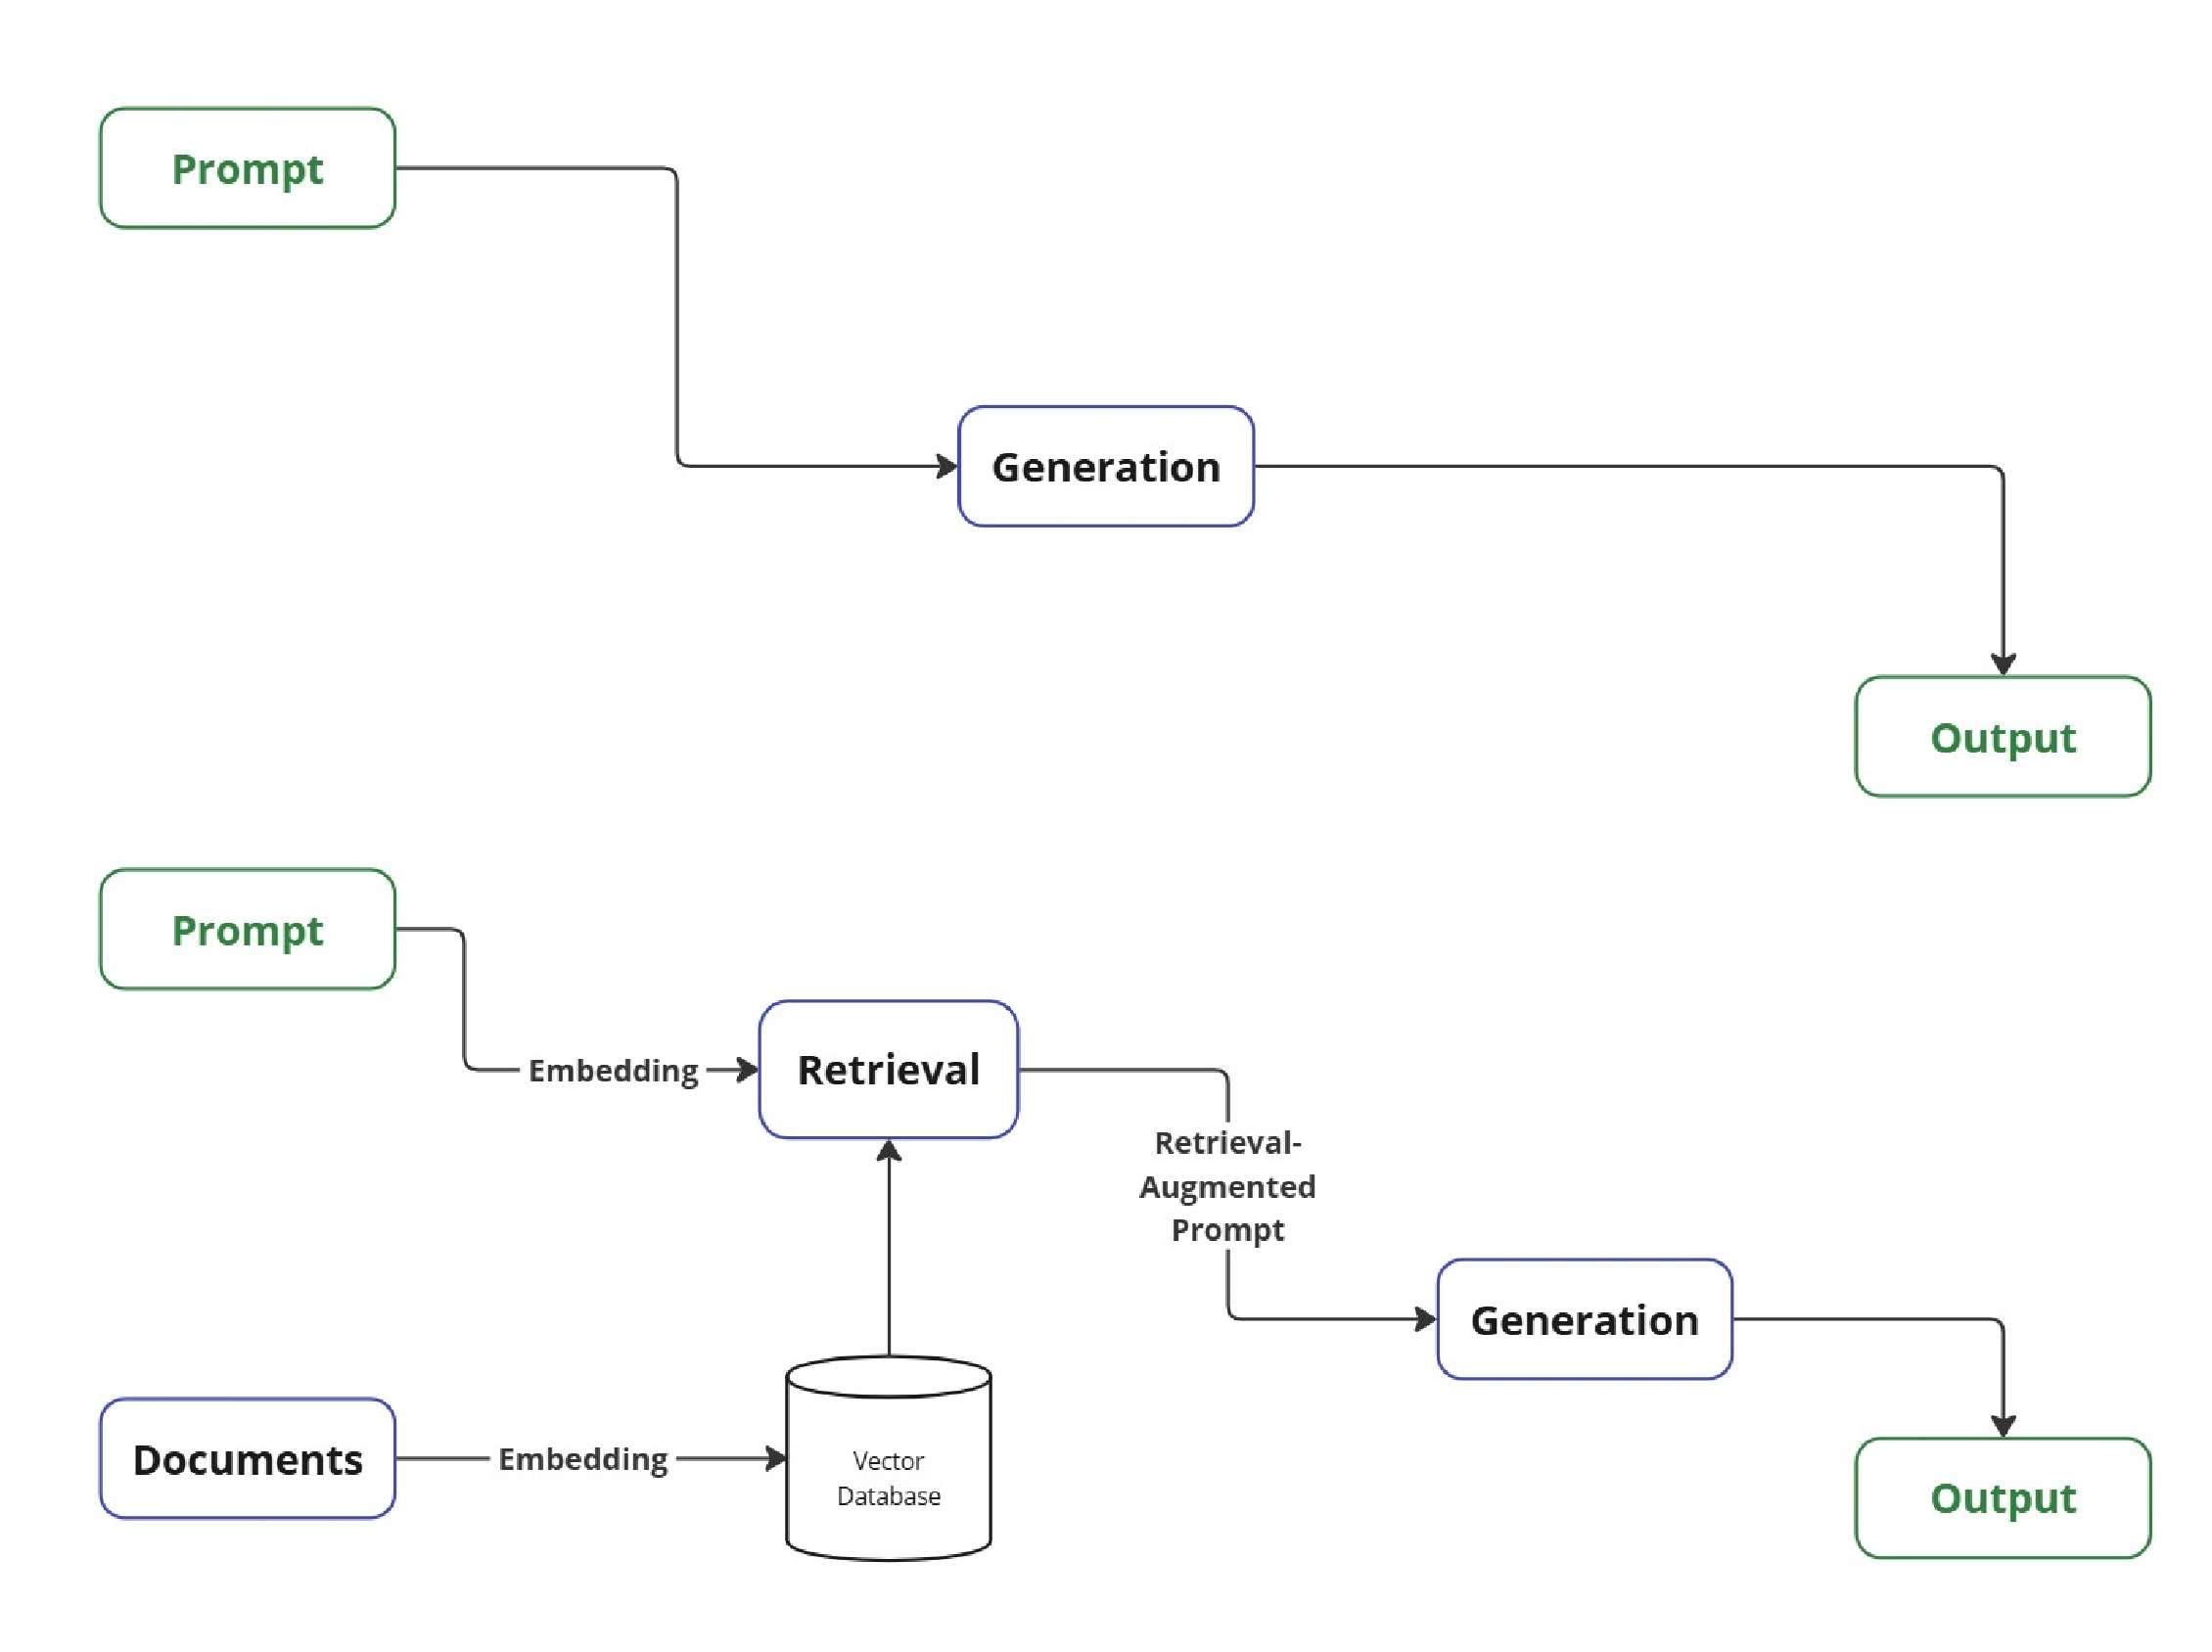
\includegraphics[width=\textwidth]{images/LLM-vs-RAG.pdf}
    \caption{Comparison of the process, above a standalone LLM that has a prompt and generate a response, below a minimalistic RAG system that performs on a given set of documents an embedding or indexing and searchs for the most similar documents for a given prompt at inference time. Both prompt and documents are used for the generation process.}
    \label{fig:naive_rag}
\end{figure}

This procedure can be seen in figure \ref{fig:naive_rag}. This generation phase is frequently termed the \textit{read} operation in literature. Gao \cite{Gao.18.12.2023} defines the naive RAG system as \textit{Retrieve-Read}. The retrieval can be done with sparse retrieval (TF-IDF, BM25), dense retrieval (DPR) or a hybrid version as showed in section \ref{retrieval}. 

\begin{figure}[h!]
    \centering
    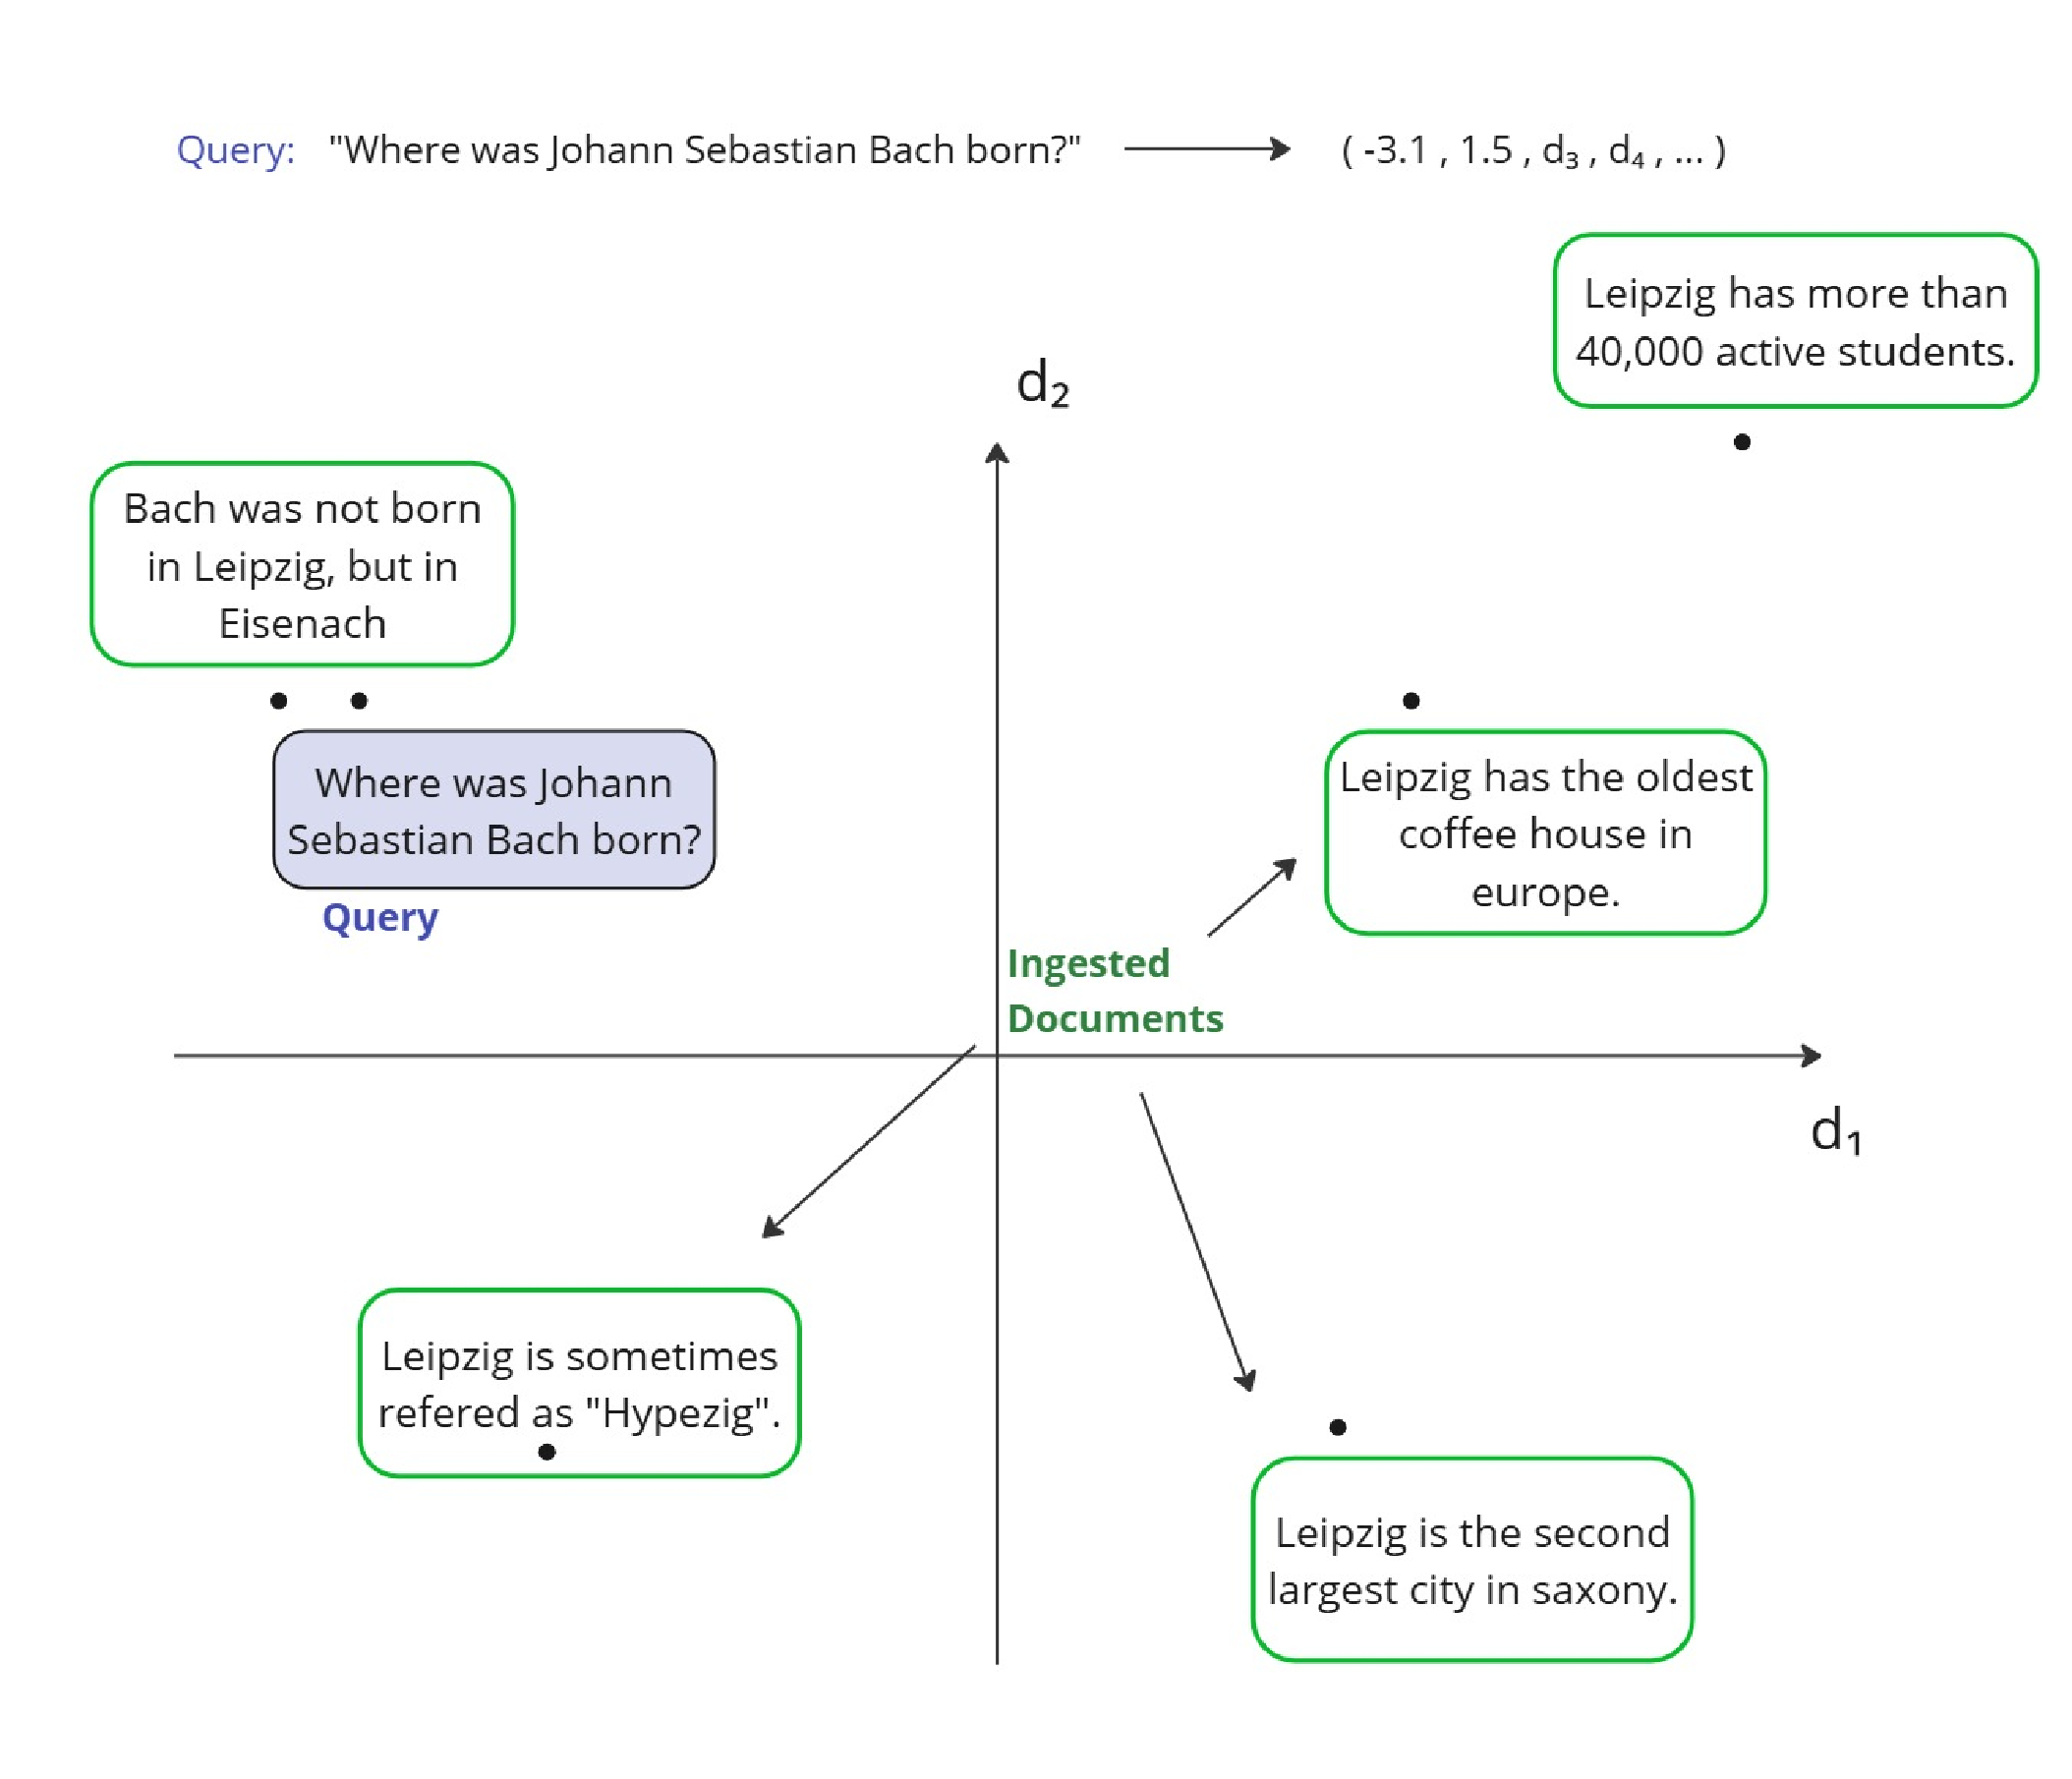
\includegraphics[width=\textwidth]{images/VectorDB.pdf}
    \caption{A vector space including mapped facts (documents) and a user query. The query and its correct answer have similar vectors}
    \label{fig:vectorDB}
\end{figure}


Before the system can be used, it is necessary to ingest data. The ingestion process includes preprocessing and selection of data, that users are likely to need for their questions or use cases. Therefore it is relevant to know the user base. It is not feasible nor efficient to ingest all availlable data. The preprocessing pipeline converts raw data into document chunks using methods detailed in Section \ref{sec:chunk}. As described in \ref{sec:dense_retrieval}, the chunks are then embedded into a d-dimensional real-valued vector space. There is a simplistic minimal example of a vector space in figure \ref{fig:vectorDB}. The documents gets mapped in different loactions within the space. This assumes semantic alignment between queries and relevant documents in the embedding space. In reality there will be more documents close to each other, documents and queries are longer or more complex and each query will return the "Top-K" chunks or documents, which are not always as relevant as in this example. Top-K can be seen as hyperparamter for the system. The vectors are then stored in vector databases, specialized databases for vector representations.
% as described in section \ref{vdbs}.


Gao \cite{Gao.18.12.2023} listed several drawbacks for naive RAGs. The basic retrieval suffers from insufficient recall and precision scores leading to irrelevant documents, missing context and bias. The integration of the provided context is a challenging process. The generator often overrelies on the augmented information by simply repeating the retrieved content and missing insightful conclusions. Therefore this simplistic form of RAG needs advanced techniques to overcome those issues.

\subsection{Advanced RAGs}
\label{sec:advanced_rags}

There is no strict definition of advanced versions of retrieval-augmented generation systems. The term describes a loose bundle of techniques to improve the quality of such systems. Following is a list, the items of which we will explain in greater detail afterwards. We will follow Gao et al. survey definition of advanced RAG that defines it as the \textit{rewrite-retrieve-rerank-read} (4R) structure with chunking enhancements. We will skip \textit{retrieve} and \textit{read} here, as we described it in section \ref{sec:naive_rags} in detail.

\paragraph{Chunking}
\label{sec:chunk}
% graphic for techniques, such as overlap, fixed sized (sliding window approach), semantic chunks, ...
Chunking's importance becomes clear through a practical example: Let us use a sentence from Wikipedia \cite{LeipzigWikipedia.2025} for Leipzig from \citeyear{LeipzigWikipedia.2025}. In the section "Music" there is the following sentence.

\begin{quote}
    "Johann Sebastian Bach spent the longest phase of his career in Leipzig, from 1723 until his death in 1750, conducting the Thomanerchor (St. Thomas Church Choir), at the St. Thomas Church, the St. Nicholas Church and the Paulinerkirche, the university church of Leipzig (destroyed in 1968)."
\end{quote}

If there are thousands of wikipedia pages or websites to process, then this can not be splitted manually. What is the document or a good chunk in this context. If the query asks if Johann Sebastian Bach lived in Leipzig, then embedding the whole sentence would not guarantee a high similarity vector score in the retrieval process. This differs from domain to domain. While chunking facts from sentences might be a valid strategy for wikipedia, processing internal contracts in a large company would need less granular chunking.

\begin{figure}
    \centering
    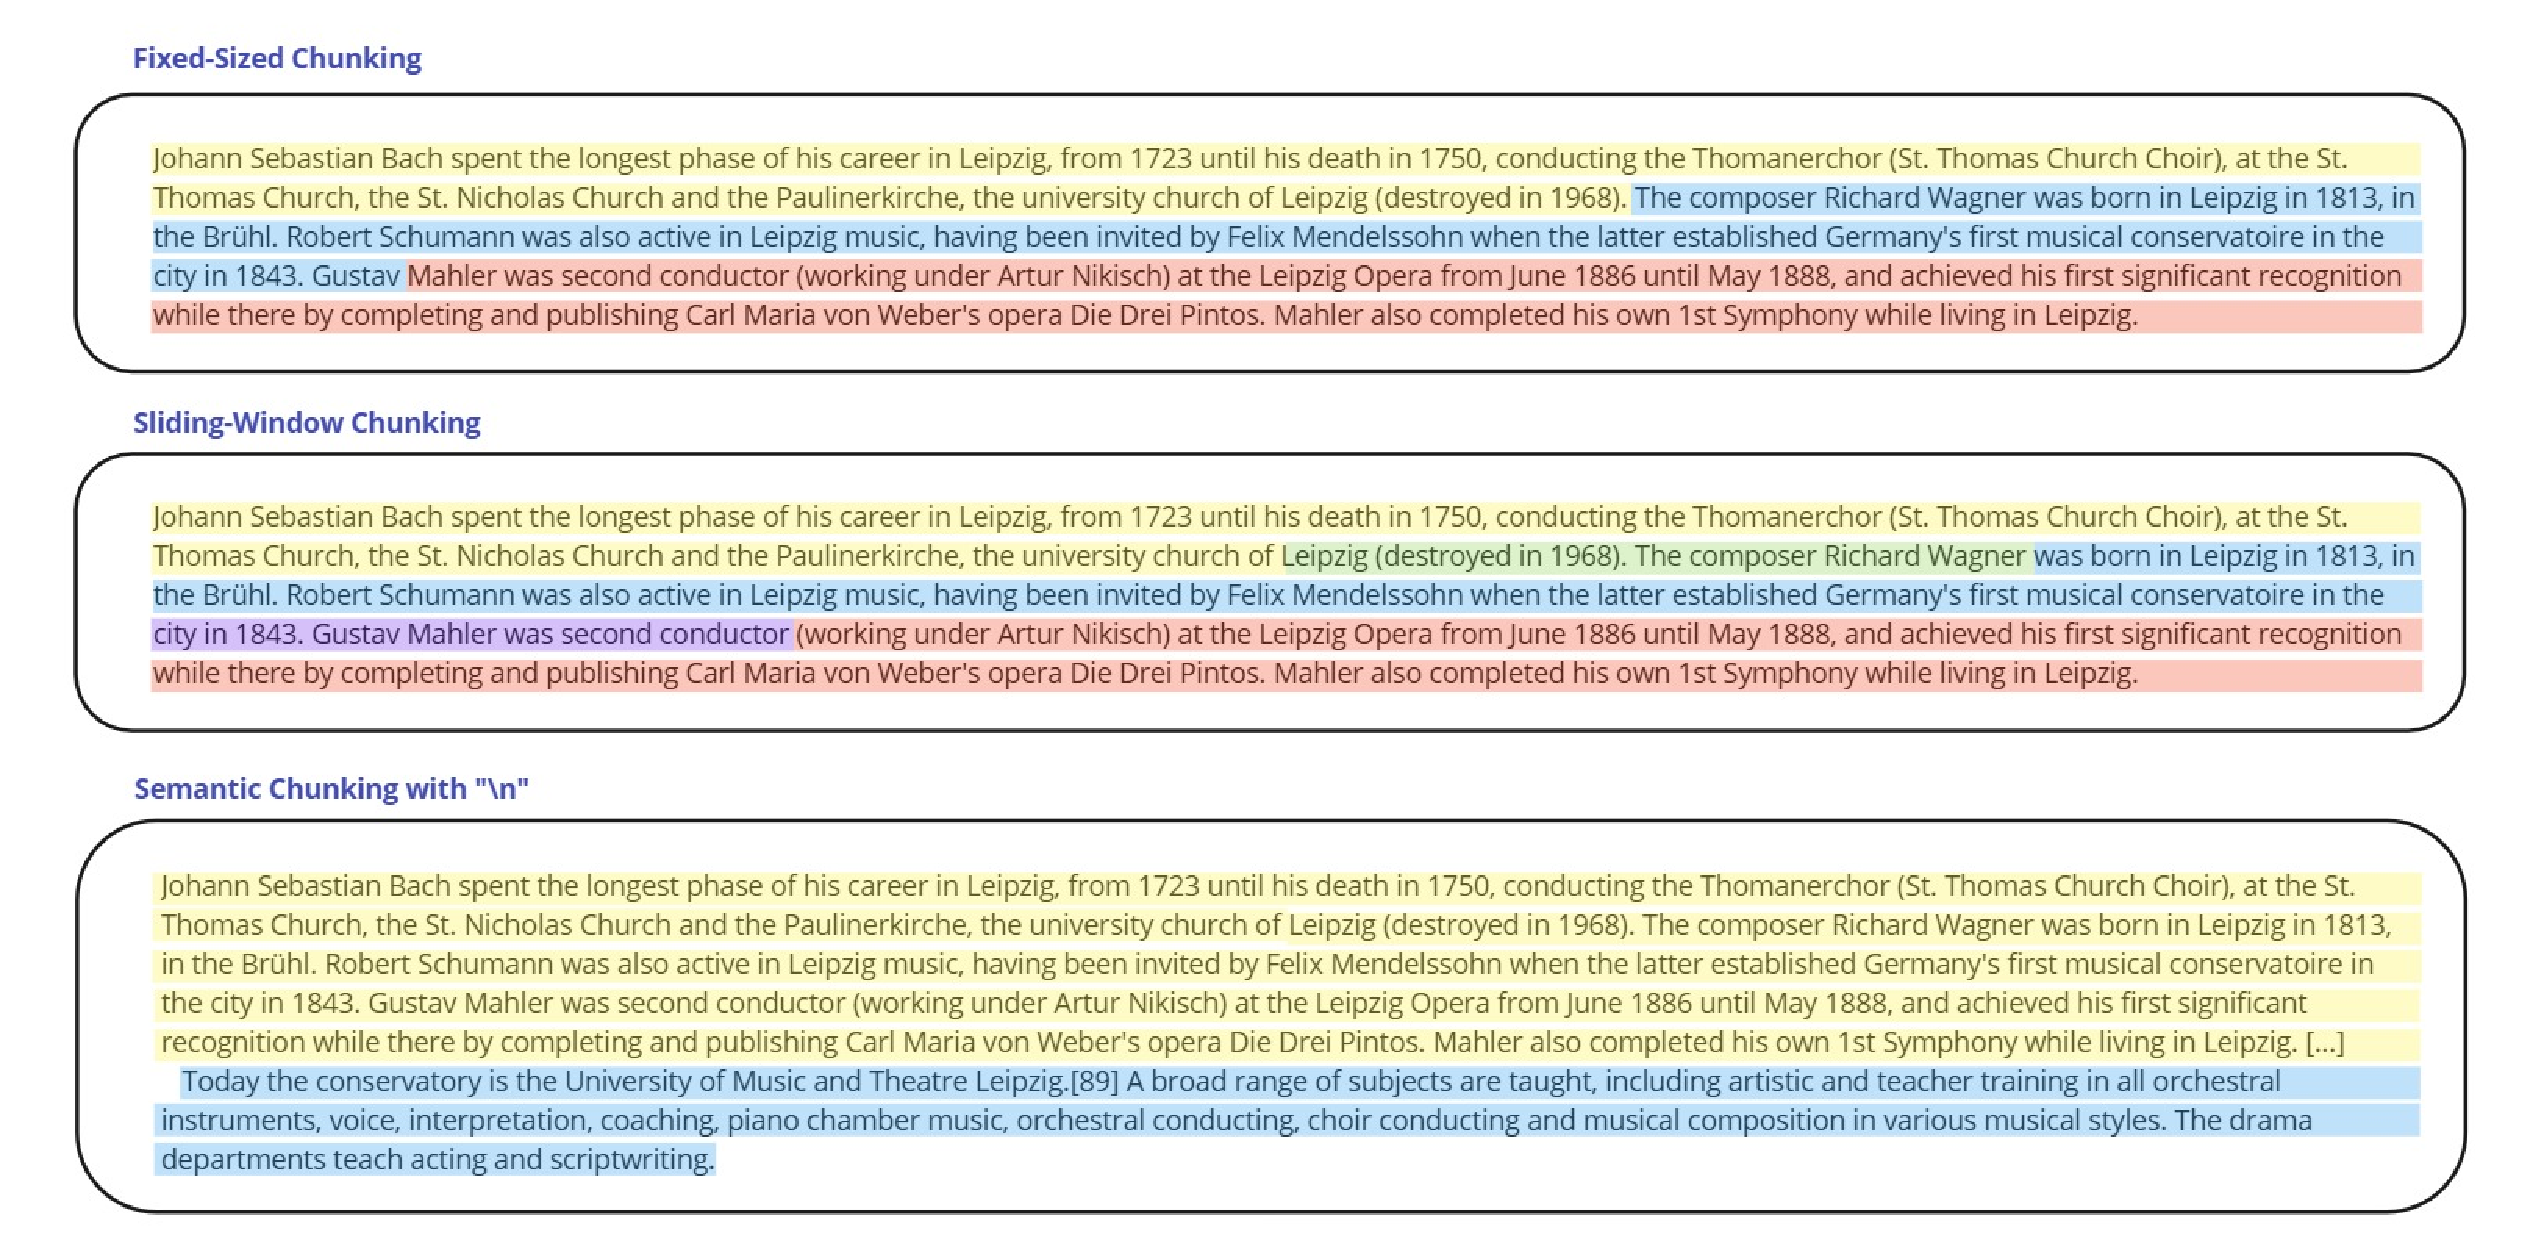
\includegraphics[width=\textwidth]{images/Chunking.pdf}
    \caption{Differnt types of chunking showed on the example of a wikipedia page of Leipzig\cite{LeipzigWikipedia.2025}}
    \label{fig:chunking}
\end{figure}

Therefore there are several chunking techniques to consider for tuning the RAG-system. Fixed-size chunking divides text into uniform segments (e.g., 400-character blocks), while sliding window variants add overlapping regions. The sliding window approach adds a overlap of few characters. Semantic chunking splits with prior defined characters such as "\textit{$\backslash n$, $\backslash\backslash n$ or <br>}". These techniques are visualized in figure \ref{fig:chunking}. There are also special use case techniques such as Markdown, JSON, HTML and programming code chunkers. Almost all presented chunking techniques are offered in typical libraries e. g. Llama-Index \cite{Liu_LlamaIndex_2022} or Langchain \cite{Chase_LangChain_2022}.


\paragraph{Rewrite}
\label{sec:rewrite}
% Query Rewriting, Query Transformation, Query Expansion (see. papers)
\textit{Rewrite} is a collection of pre-retrieval techniques to increase the likelihood of relevant retrieved documents and a concise generation. The query will be transformed, expanded or routed. Query routing in this context describes different RAG pipelines based on the query.\cite{Gao.18.12.2023}

\paragraph{Rerank}
\label{sec:rerank}
% Reranking Techniques, Lost-in-The-Middle?, Diversity Ranking, ...
\textit{Reranking} mitigates risks from which naive RAGs suffer. The key consideration for retrieval is deciding how many documents should be retrieved. In real worlds scenarios there won't be perfect retrievals. Therefore the retrieval will always introduce noise in form of irrelevant documents or chunks into the generation process. Additional to this, if we retrieve not enough documents, we might risk losing relevant ones that do not appear at the top of the similarity score. Post-retrieval techniques such as reranking mitigate this risk by ranking and ordering those documents.\cite{Gao.18.12.2023}


\section{Modular RAG}

There is a variety of different RAG systems with lots of different components. The definition of advanced RAG systems is too strict and sequential for including this variety. Modular RAGs close this gap. Modular RAGs can be seen as individual component blocks that can be added to a pipeline as long as the input and output of these blocks are compatible. Gao et al. introduced this definition and defined more components then the here presented \textit{rewrite, retrieve, rerank and read}.\cite{Gao.18.12.2023} One simple example of the need for modular RAGs is a routing component, that decides if retrieval is necessary at all. Redirecting to the generator can lead to less computational time and better results in some cases.\cite{Mallen.20.12.2022} This modularity is a key requirements for the ability to build custom RAG systems for each use case.


\subsection{Drawbacks of RAGs}
\label{sec:drawbacks}
Retrieval-augmented Generation systems have several improvements compared to standalone LLMs as described at the beginning of this chapter. Nevertheless, it comes with drawbacks that must be considered before replacing LLMs in production.

\begin{enumerate}
    \item RAGs have significantly longer computation times and must be partially computed in sequential order. Therefore the time-to-first-token (TTFT) is always higher then the vanilla LLM.
    \item This increase in computation times and the fact that there are more LLM requests for e.g., rewriting or reranking result in higher costs.
    \item RAGs introduce an overhead of work and expertise for developing, maintaining, and experimenting with RAGs.
    \item RAGs introduce a wide variety of diverse failures in all components of the RAG system. Failures can happen while ingestion too.
\end{enumerate}

These points show that RAGs are no free lunch, and it must be considered if RAG is needed for every specific use case. Therefore, there is a need for fast RAG experimentation that can address all points necessary for this decision.
